\subsection{Ecuador}\label{subsec:ecu}

The WCD prototype ``Chimbito'' was installed in August $2012$ at Escuela
Polit\'{e}cnica del Chimborazo (ESPOCH) at $2870$~m a.s.l, which is about $60\
{\rm km}$ from the Chimborazo volcano.

\subsection*{Detector Prototype}

We use a commercial water tank, with a capacity of about 1100 l, and low
cost accessories to build the detector system. From bottom to top, the tank is
mostly cylindrical, followed by a truncated-cone section and a cylindrical end
at the top. The radius of the base of the main cylinder is 55\,cm, and its
height 110\,cm. The upper cylindrical part, which hosts the water tank cap, has
a diameter of 50\,cm and a height of 11\,cm. A detailed drawing can be seen in
Fig. \ref{fig:ecuador-tank}, left.

\begin{figure}[!ht]
  \centering
 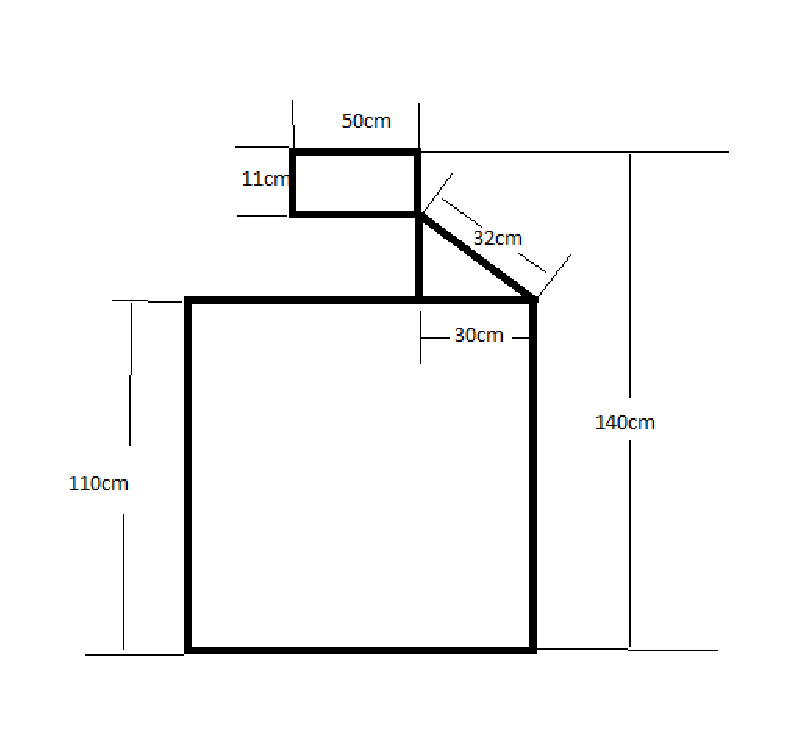
\includegraphics[width=0.45\textwidth]{images/ecuador/chimbito_dimensiones}
 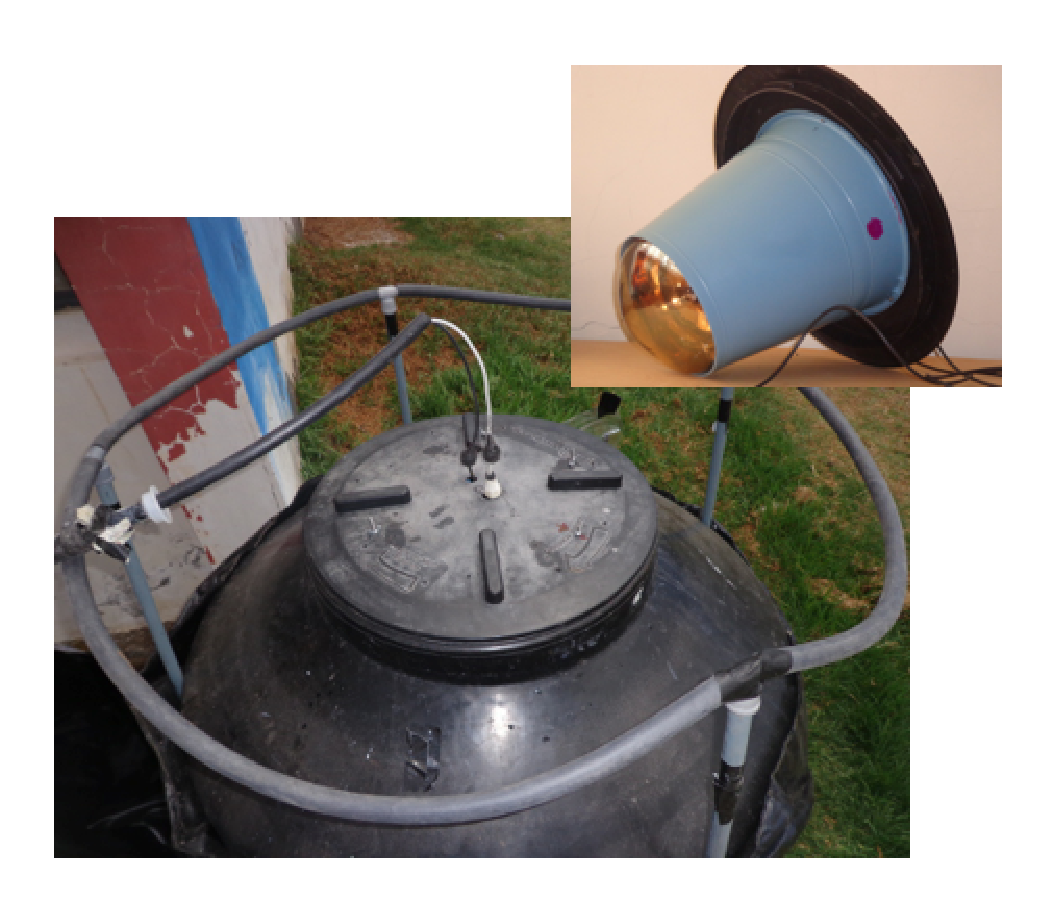
\includegraphics[width=0.45\textwidth]{images/ecuador/icrc2013-1208-01}
  \caption{Left: Dimensions of the WCD. Right: WCD prototype ``Chimbito'' installed at Riobamba, Ecuador. The PMT and its support are shown in the inset.}
  \label{fig:ecuador-tank}
 \end{figure}

The external walls of the tank are protected with four layers of high-density
non reflective black polyethylene. To guarantee good reflectivity and
diffusivity, the internal walls of the tank are lined with Banner-type
material. We also use Tyvek$^{\textregistered}$ as inner lining material
supported by a frame inside the tank and floating on top of the water. A
Photonis XP1802 9'' PMT is mounted for the Cherenkov light collection and
is placed at the top and central part of the detector cap. A hole was cut on
the Tyvek$^{\textregistered}$ surface in order for the PMT to protrude into the
inner part of the tank. The PMT is connected to a digitizer board and a FPGA,
whose connection was developed by the Bariloche group. The prototype is shown
in Fig. \ref{fig:ecuador-tank}, right. Special care has been taken to isolate this device
and its electronics board from moisture and to avoid water entering the PMT
hose. 

The shock chlorination technique has been used to improve the quality and
purity of the water. This process consists of the dilution of a high
concentration of chlorine Cl$_{2}$ into the water (approximately 150 mg of
Cl$_{2}$ per liter) in order to purify it. This method allows very low light
absorbance in a spectral range from $350$ to $750$\,nm. However, due to its low
cost and relatively easy way to apply, it has been chosen as the default method
of purification. It is important to mention that it is the first time that this
process is used to purify water for WCD in the LAGO Collaboration. Furthermore,
Amino-G, ${NH_{2}C_{10}H_{5}(SO_{3}H)S)_{3}Na}$, the most common wavelength
shifter used in water Cherenkov detectors, has been added to the water in a
concentration of $1$\,mg per liter. Studies report that, with this addition,
the efficiency of the detector increases by a factor of 3 without loosing the
directionality of Cherenkov light \cite{Badino1981}.

\subsection*{Operational Status of the Detector}

In the top panel of figure \ref{fig:results-ecu}, it is shown an individual
pulse and the mean signal response of the detector for data taken in September
2013.

 \begin{figure}[!ht]
  \centering
 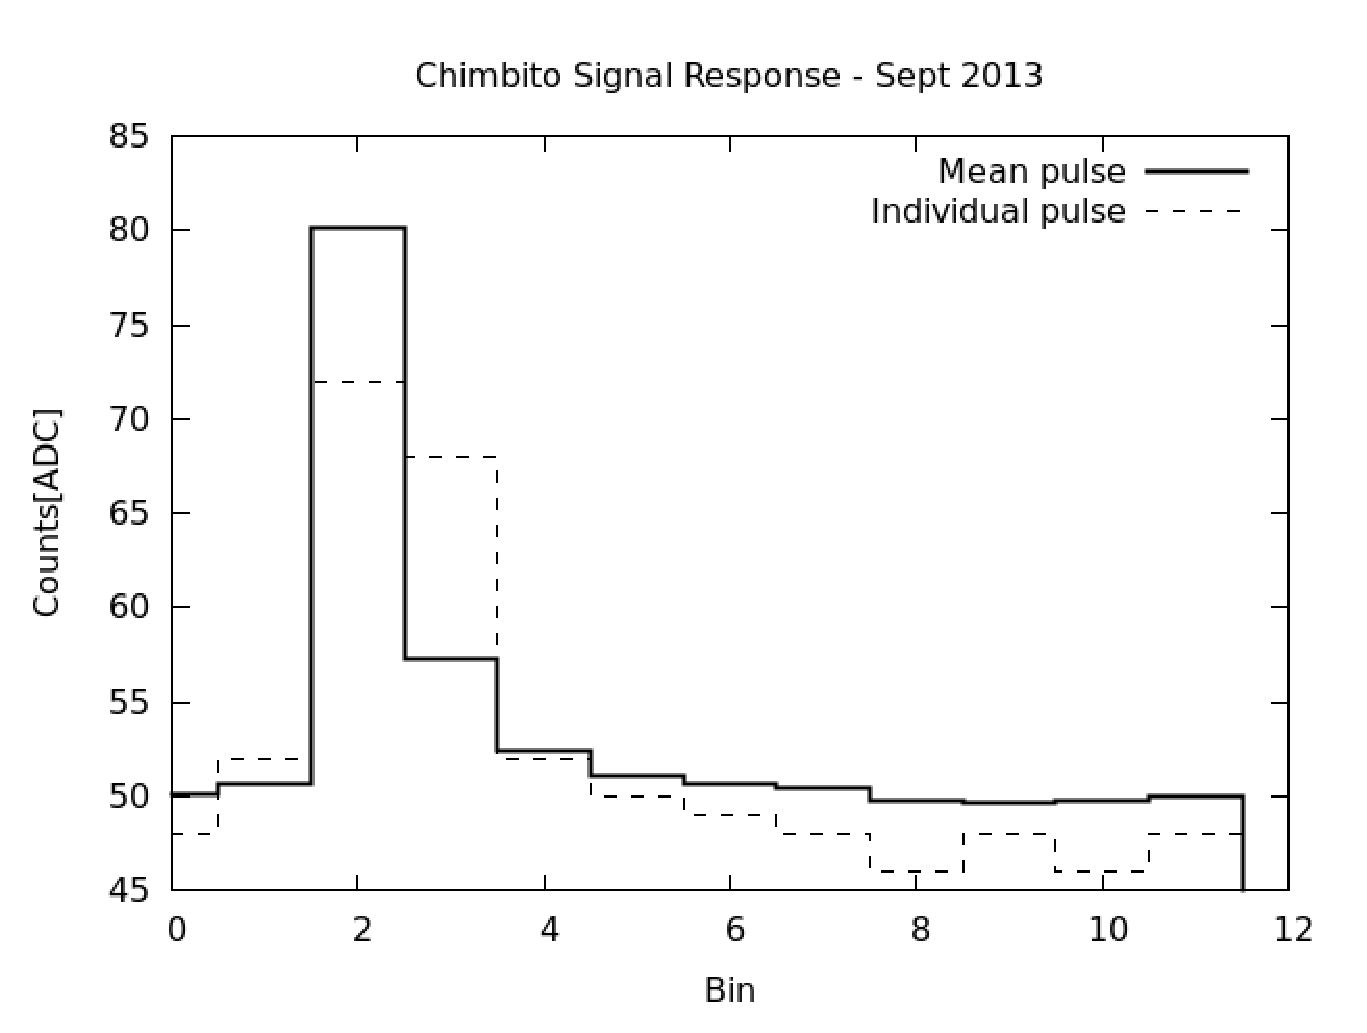
\includegraphics[width=0.8\textwidth]{images/ecuador/promedioSep21h}
 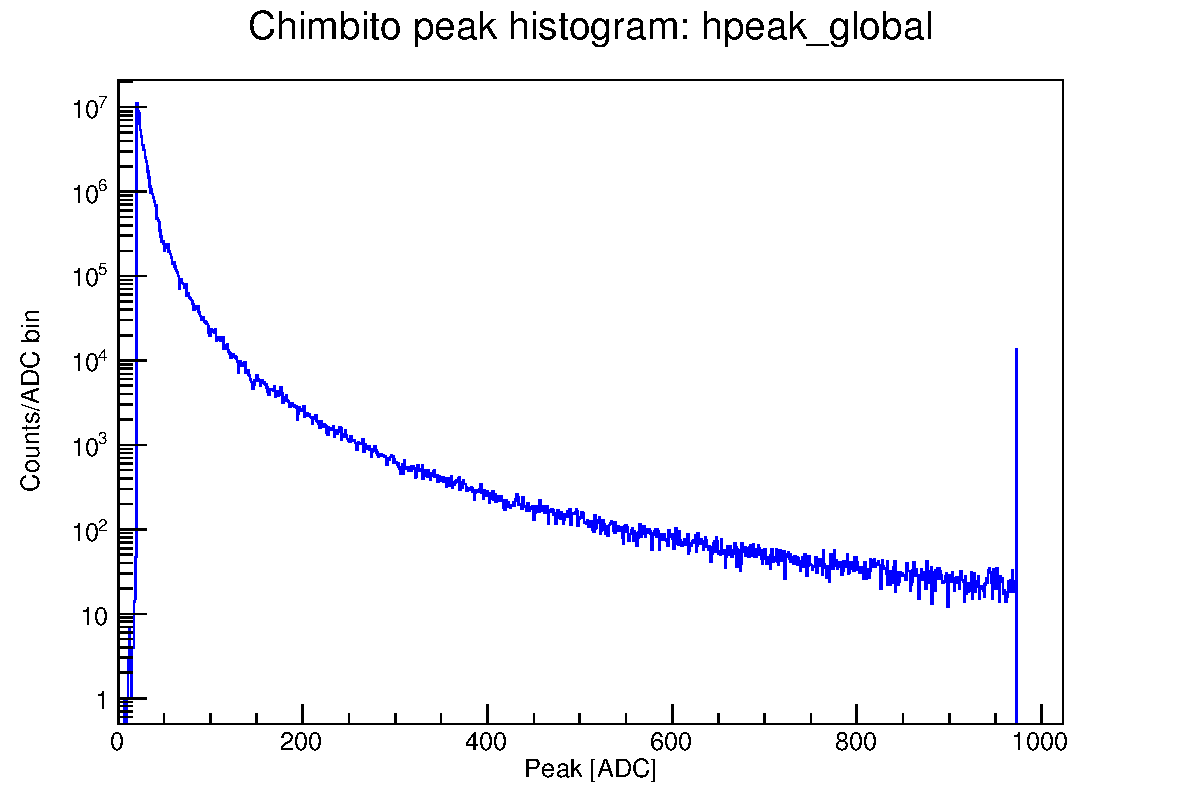
\includegraphics[width=0.49\textwidth]{images/ecuador/peak_histo_chimbito_jul_nov_2013}
 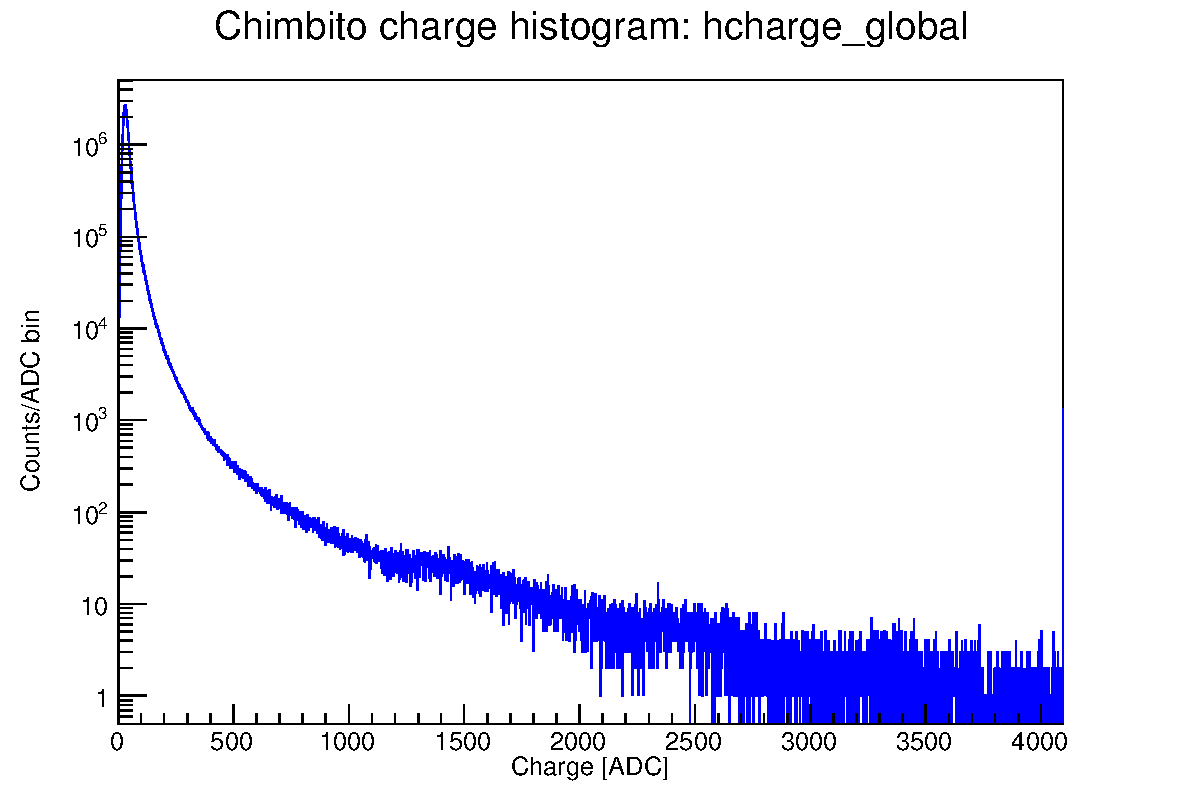
\includegraphics[width=0.49\textwidth]{images/ecuador/charge_histo_chimbito_jul_nov_2013}
  \caption{Top: mean signal response ``Chimbito''. The individual signal response of a pulse is also shown. Bottom left: Peak histogram with data taken between July and November 2013. Bottom right: charge histogram with data taken between July and November 2013.}
  \label{fig:results-ecu}
 \end{figure}

Calibration histograms have been extracted from the collected data. A total
charge histogram and a peak histogram for data collected between July and
November of $2013$ are shown in bottom right panel and bottom left panel of
figure \ref{fig:results-ecu}, respectively. 

Currently, all the flowing data is being analyzed and interpreted in order to
understand the performance of the detector and to identify any possible changes to
the hardware configuration. The calibration of the detector using the muon peak
is expected to be done in a short time.

In the near future, the final objective is to locate a new detector in the
Chimborazo snowcap foothills at 4800 m a.s.l., which will be, to our
knowledge, the second highest LAGO site after Chacaltaya (see table \ref{tab:locations}),
Bolivia. The data taken from this new detector is expected to be compared with
the data obtained with the ``Chimbito'' detector. Due to the high altitude of
this site  this comparison could increase the detection sensitivity of
transient events emitting high energy photons.

It is worth mentioning that a new WCD prototype ``Panchito'' is under
construction at Cumbaya, Quito (2398 m a.s.l.), Ecuador. This detector will be
located at Universidad San Francisco de Quito (USFQ). We will use a commercial
water tank of 2500 l similar to the one used in ``Chimbito'' design but with a
geometry better suited for photon detection. The radius of the base of the main
cylinder is 78.4\,cm, and its height 146\,cm. The upper cylindrical cap has a
diameter of 55\,cm. The internal walls of the WCD will be covered by
Tyvek$^{\textregistered}$ and Banner-type material in a manner similar to the
detector in Riobamba. The PMT XP1802 9''produced by Photonis will be connected
to an acquisition board. It has sensitivity over a wide spectral range, from
270 to 650\,nm.

A new high altitude site near the east side of Pichincha Volcano, Cruz Loma at
4100 m a.s.l., is also under consideration. This detector is expected to be used
for high energy physics analysis. Meanwhile, ``Chimbito'' and ``Panchito''
detectors will be used for solar physics analysis and software development.
Multiple comparisons could be done using the data obtained with this detector
array.
